%!TEX root = ../../thesis.tex
\section{Continuous state space}
\label{chapter:limitations:continousstate}

\question{How to leverage from the discrete set of state constrain?}

In this section we extend our algorithm to a more complex scenario by considering a continuous world, more complex reward functions and the use of both feedback and guidance instructions. We investigate how our algorithm scales to such problem and how different exploration strategies perform.

\subsection{Experimental System}

We now illustrate the application of our algorithm in a more complex problem. This problem is known in the reinforcement learning literature as the \emph{puddle world}. The puddle world consist in a continuous-state MDP in which an agent must reach a goal region while avoiding a penalty region.
% 
In this work we consider a 2 dimensional puddle world with each dimension ranging between 0 and 1. Agent actions are discrete and represent steps in either North, South, East, West direction. One step length is sampled from a normal distribution of mean 0.1 and standard deviation 0.01.

As in the previous experiment, we consider speech as the modality for interacting with the robot and we reuse the dataset used in section~\ref{sec:First}. The interaction scheme is turn taking, where the agent is performing an action and wait for a feedback or guidance signal to continue (see section \ref{sec:mixing}). We only consider a Gaussian classifier.

\subsubsection{Task Representation}
To define the set of possible tasks we project a 5x5 regular grid on top of the continuous world. One task is represented by a +1 reward in one of the 25 projected squares and a -100 reward in three consecutive (vertically or horizontally) squares. +1 and -100 area can not overlap (see figure~\ref{UncertaintyMap}(E) for an example). The set of possible task is defined as all possible combination of such reward function, for a total of 660 hypothesis. 

We use the MDP framework to compute the corresponding policies. The world being continuous we use the tile coding function approximation \cite{sutton1998reinforcement}, with 10 overlapping 50x50 regular grids. %tillins. 
A Q-Learning algorithm \cite{watkins1992q} is used to compute the Q-Values, with a discount rate of 0.99 and a learning rate of 0.01. The hypothesis policies are then defined as greedy according to the Q-Values.

\subsubsection{Exploration strategies}

We will investigate four different agent behaviors. 1) random, 2) $\epsilon$-greedy, 3) myopic uncertainty based exploration, which aim at selecting the action that is the most uncertain in the current state, and 4) full uncertainty based exploration which requires an uncertainty map to decide what to explore next, as presented in Section~\ref{sec:Planning}. 

As we are in a continuous domain we can not compute the full uncertainty for each state as presented in Section \ref{sec:ExplorationMethod}, we therefore approximate this process. Extensions already exist for the continuous state problem \cite{nouri2010dimension,Hester13aamas} and we will rely on a sampling based method. One hundred random states are generated and evaluated in terms of task and instruction uncertainty as described in Algorithm~\ref{alg:u}. Each sampled state is associated to a reward value proportional to its uncertainty which is propagated to neighborhood states by using a fixed Gaussian kernel. We use as amplitude the uncertainty value and a diagonal covariance matrix of value 0.01. The resulting approximated uncertainty map is then used as a reward function in a new MDP problem. By solving this problem, using for instance Q-Learning, the agent plans actions to visit the most uncertain regions. The system can then run an $\epsilon$-greedy policy on this solution. In the following experiment, the agent will use an exploration ratio $\epsilon$ equal to $0.1$.

\subsubsection{Feedback and Guidance Model}
\label{sec:advancedModel}


\subsection{Mixing feedback and guidance}
\label{sec:mixing}

The previously defined teaching signal model limits the use of only feedback or only guidance instruction. Such limitation can be restrictive for the user, we will now consider the case where teachers can use both, i.e. $z \in \{F \cup G\}$. Extending our algorithm to cases where possible meanings include both feedback and guidance requires a probabilistic model of how the teacher distribute feedback and guidance signals. This model must hold the following property $\sum_{i \in \{F \cup G\}} p(z = i|s,a,\hat{\xi})~=~1$. We define a variable $\beta$ that represents the probability of the user providing a feedback signal at each step, i.e. $p(z \in F) = \beta$, which implies $p(z \in G) = 1 - \beta$. 

In \cite{macl11simul} the agent was estimating such protocol parameters from the interaction. In this work we will assume such parameter is known in advance (see Section~\ref{sec:advancedModel}) and further assume it does not depend on the task or on the state of the robot. 
%
Under this new definition we can change the likelihood function to:
%
\begin{eqnarray}
\L_i &=&  p(n_i|s_i,a_i,\hat{\xi},\theta)\nonumber\\
%               &=& \sum_{j} p(n_i|z = j,s_i,a_i,\hat{\xi},\theta)~p(z = j|s_i,a_i,\hat{\xi},\theta)    \nonumber\\
                &=& \sum_{j} p(n_i|z = j,\theta)~p(z = j|s_i,a_i,\hat{\xi}) \nonumber\\
                &=& \sum_{j} p(n_i|z = j,\theta)~w_{ij}^{\hat{\xi}}
                \label{eq:likmix}
\end{eqnarray}
%
with :
%
\begin{eqnarray}
    w_{ij}^{\hat{\xi}} = 
        \begin{cases} 
            \beta~p(z|s_i,a_i,\hat{\xi}) &\mbox{for } z \in F \\
            (1- \beta)~p(z|s_i,\hat{\xi}) & \mbox{for } z \in G
        \end{cases}
        \label{eq:mixedfeedbackguidance}
\end{eqnarray}

We consider both feedback and guidance instruction simultaneously. Extending our algorithm to cases where possible meanings include both feedback and guidance requires a probabilistic model of how the teacher distribute feedback and guidance signals. We will use the mixing model described in Section~\ref{sec:mixing} with the individual feedback and guidance model as describe in Section~\ref{sec:fisrtFrame} and a mixing ratio $\beta$ of 0.5. It means that the user is expected to deliver feedback and guidance signals at a similar rate.


\subsection{Results}

We present results from 75 runs of our experiment, where for each run we randomly choose a task to teach from the set of hypothesis as well as the initial state of the agent. For each experiment, we compute the likelihoods every 15 steps and performs a total of 35 updates, for a total of 525 iterations. Figure~\ref{Rmax} shows the average evolution of the taught task hypothesis likelihood.

\begin{figure}[!htbp]
  \centering
  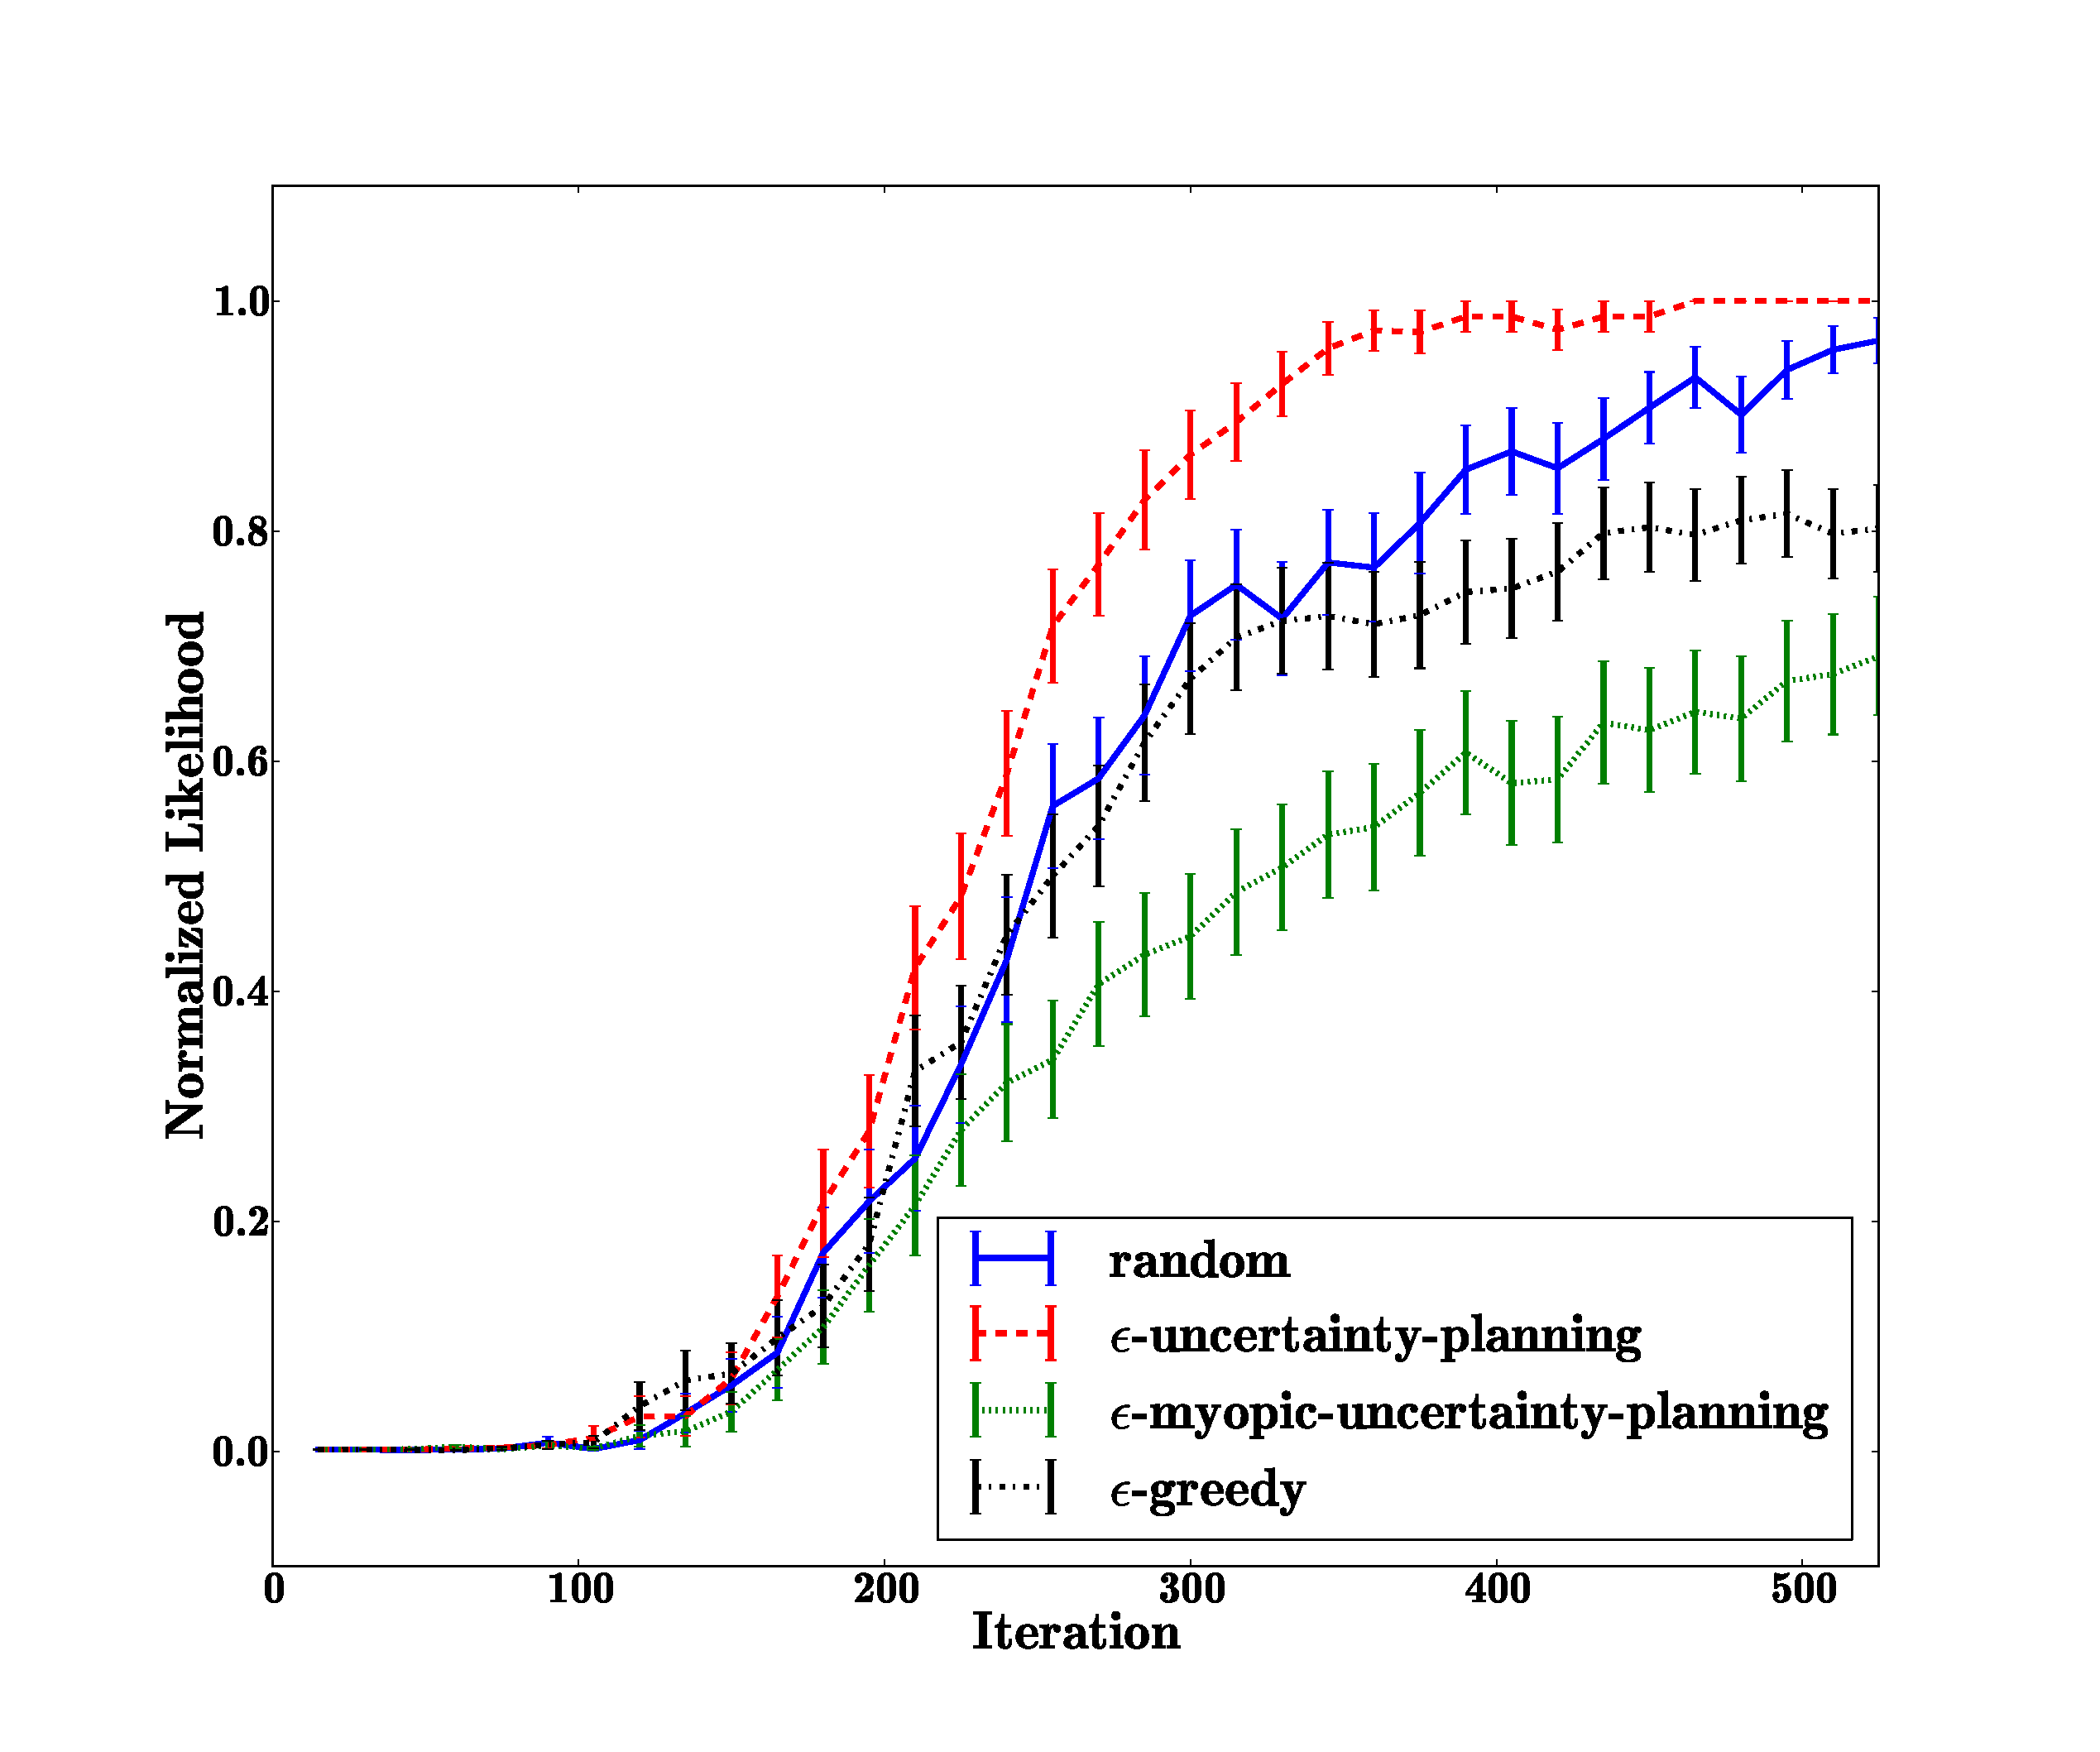
\includegraphics[width=\plotsize\columnwidth]{\imgpath/continuous_state/continuous}
  \caption{Taught hypothesis normalized likelihood evolution (mean + standard error) thought iteration using Gaussian classifer. Comparaison of different exploration strategies. Uncertainty based exploration method, which plan on the long term, performs significantly better.}
  \label{Rmax}
\end{figure}

Results from figure~\ref{Rmax} show that our algorithm can learn a task in a continuous world from unknown and noisy instructions whose possible meanings are both feedback and guidance and 10\% of the instructions were teaching mistakes. The uncertainty based planning strategy outperforms random action selection. Interestingly, myopic uncertainty based strategy, which is also based on both task and signal uncertainty, is not efficient. This result illustrates some of the issues discussed in section~\ref{sec:Planning}, when considering the agent as not being able to teleport, long term planning is more suited to explore efficiently the state space. 

As expected $\epsilon$-greedy performs less efficiently than in the first setup. This is due to the properties of our new set of hypothesis where many hypothesis shared an identical positive reward area but have different puddle zone.

Figure~\ref{UncertaintyMap} shows the evolution of the estimated uncertainty map for one run of the experiment. For each uncertainty map, the agent plans its actions to reach a maximal uncertainty region. The maximum uncertainty value decreases as the agent is correctly estimating the task.

\begin{figure}[!htbp]
  \centering
      \begin{subfigure}[b]{0.35\columnwidth}
          \centering
          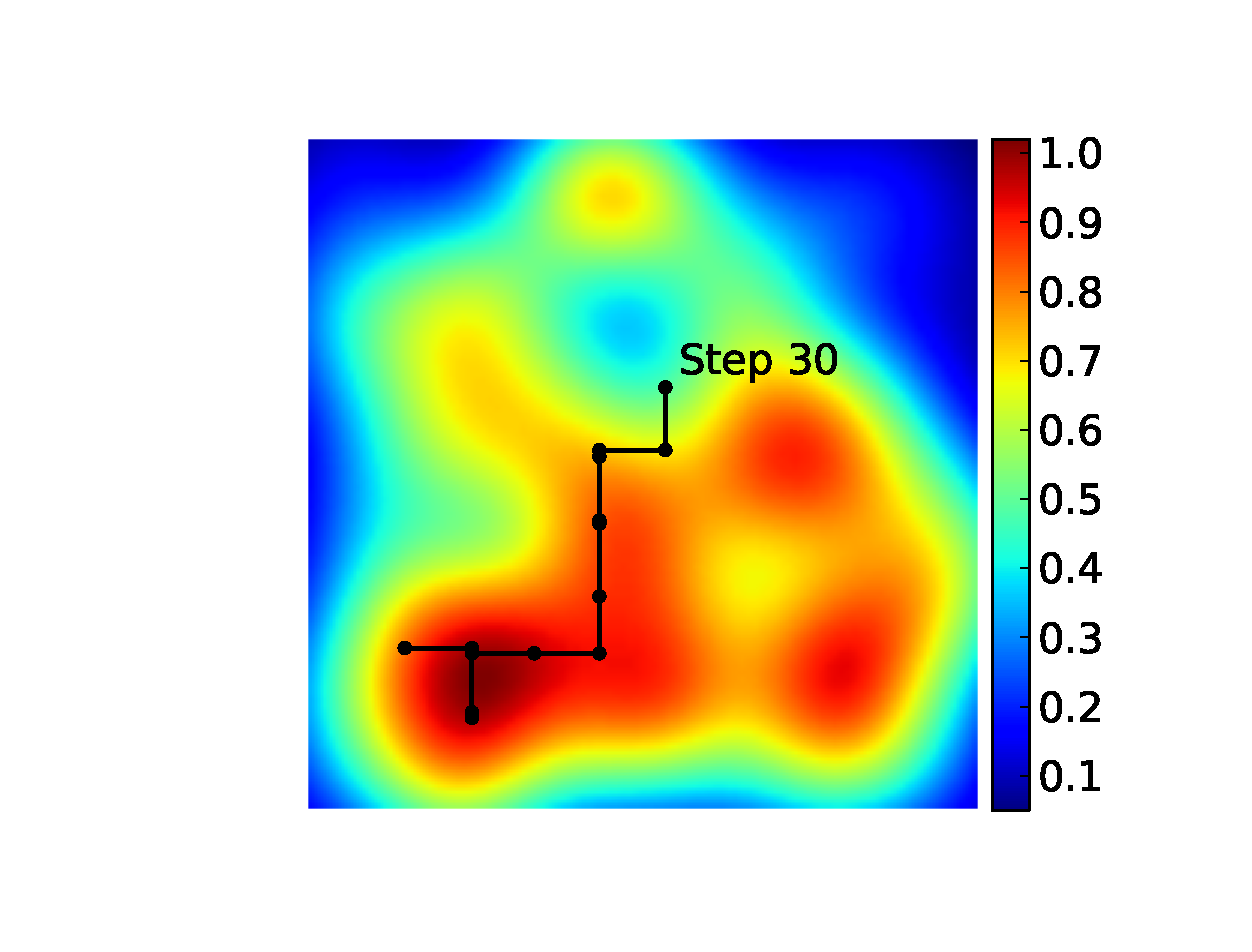
\includegraphics[trim=5cm 1.5cm 1.5cm 1.5cm, clip=true, width=\columnwidth]{\imgpath/continuous_state/30}
          \caption{After 30 iterations.}
          \label{fig:30}
      \end{subfigure}
      \begin{subfigure}[b]{0.35\columnwidth}
          \centering
          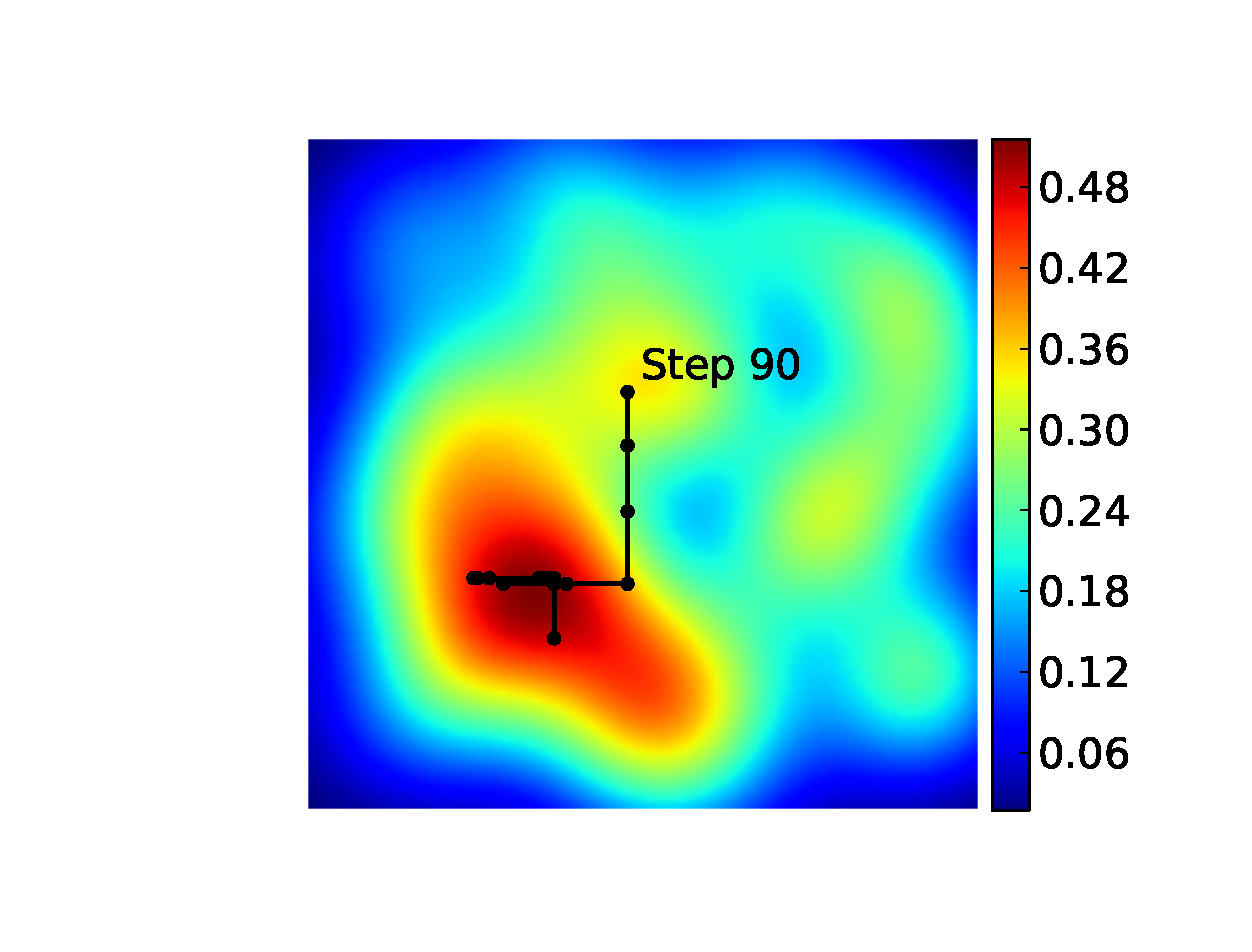
\includegraphics[trim=5cm 1.5cm 1.5cm 1.5cm, clip=true, width=\columnwidth]{\imgpath/continuous_state/90}
          \caption{After 90 iterations.}
          \label{fig:90}
      \end{subfigure}\\
      \begin{subfigure}[b]{0.35\columnwidth}
          \centering
          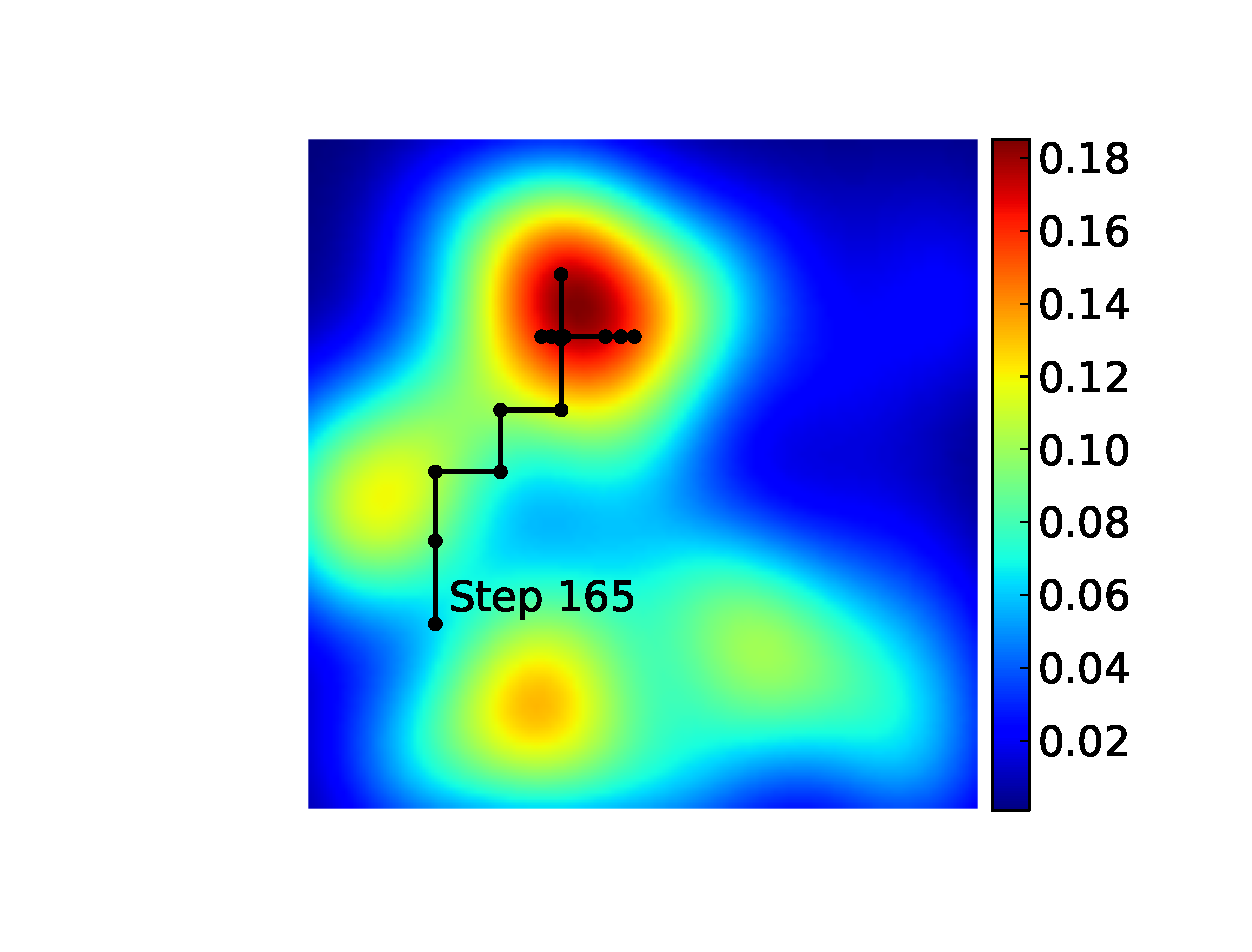
\includegraphics[trim=5cm 1.5cm 1.5cm 1.5cm, clip=true, width=\columnwidth]{\imgpath/continuous_state/160}
          \caption{After 165 iterations.}
          \label{fig:165}
      \end{subfigure}
      \begin{subfigure}[b]{0.35\columnwidth}
          \centering
          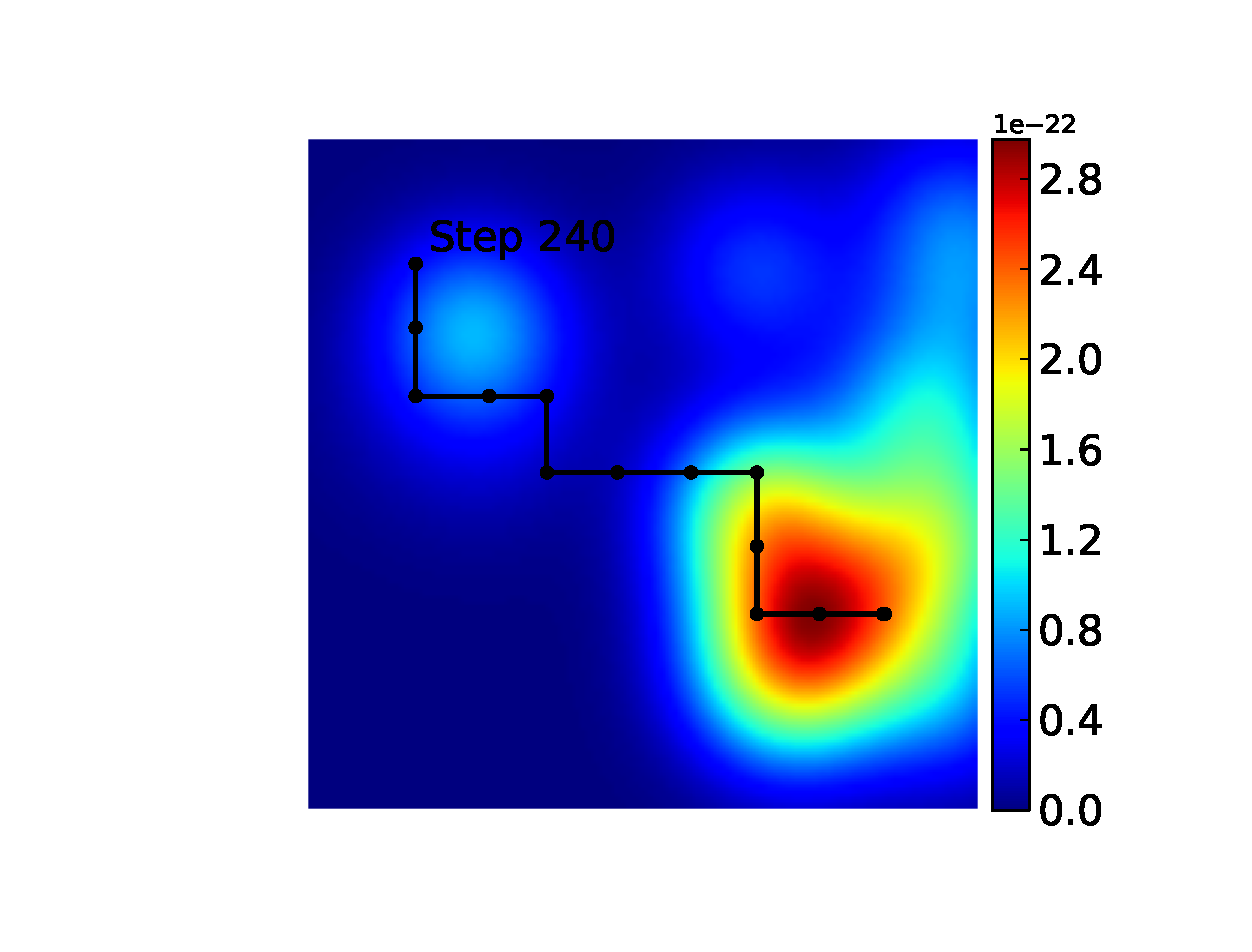
\includegraphics[trim=5cm 1.5cm 1.5cm 1.5cm, clip=true, width=\columnwidth]{\imgpath/continuous_state/240}
          \caption{After 240 iterations.}
          \label{fig:240}
      \end{subfigure}\\
      \begin{subfigure}[b]{0.25\columnwidth}
          \centering
          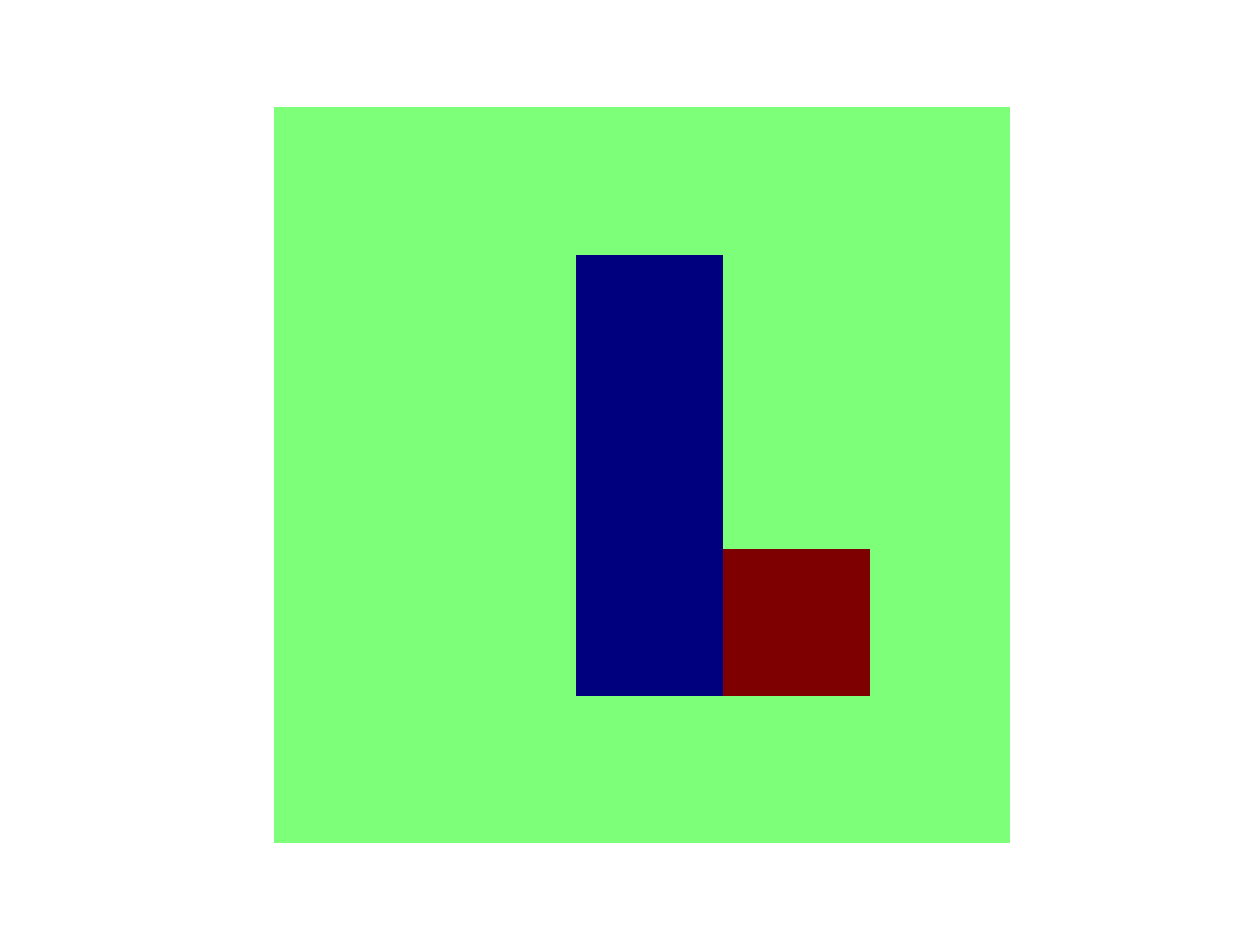
\includegraphics[trim=4cm 1cm 3.5cm 1cm, clip=true, width=\columnwidth]{\imgpath/continuous_state/puddle}     
          \caption{Puddle world used by the teacher.}
          \label{fig:puddle}
      \end{subfigure}
      \begin{subfigure}[t]{0.45\columnwidth}
          \centering
          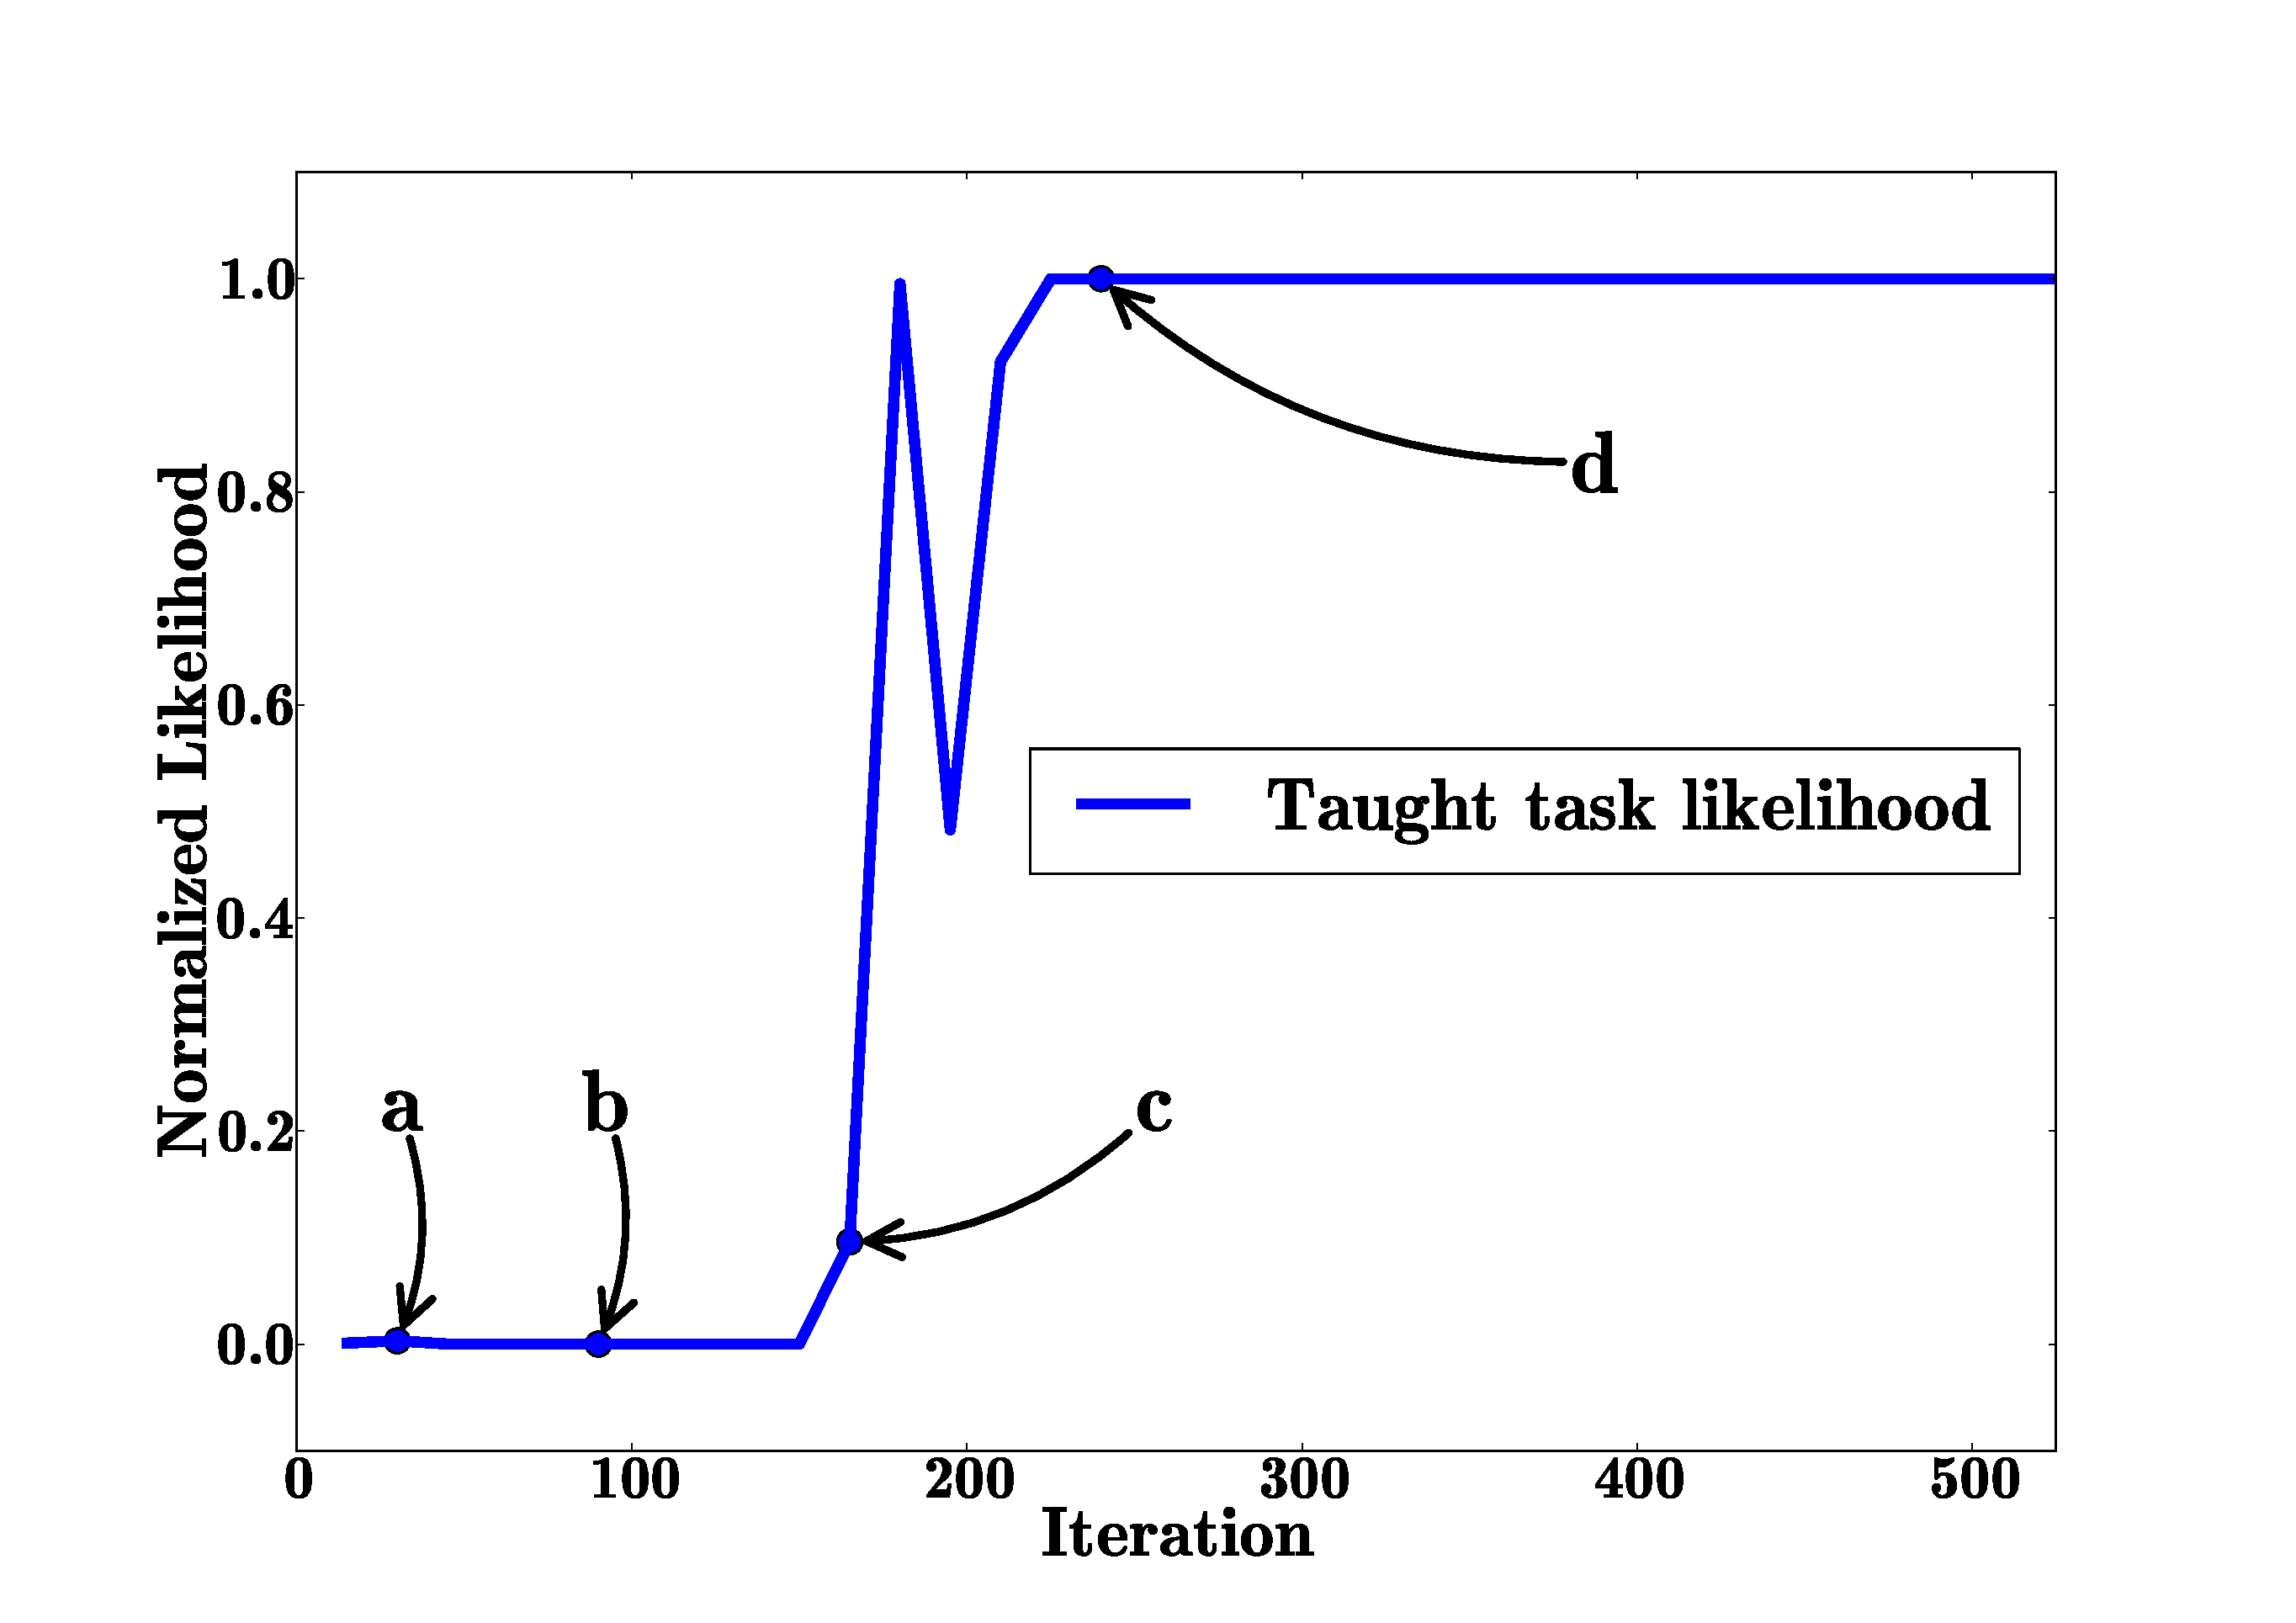
\includegraphics[trim=2cm 1cm 3cm 2cm, clip=true, width=\columnwidth]{\imgpath/continuous_state/evo}
          \caption{Taught hypothesis normalized likelihood evolution.}
          \label{fig:evo}
      \end{subfigure}
        
  \caption{Log Uncertainty maps after a) 30, b) 90, c) 165 and d) 240 iterations. e) shows the puddle world choosen by the teacher and f) shows the learning progress and the frame associated to each of the uncertainty map. In order to display the differences between log values, we bounded the colormap between -5 and 0, which correspond to uncertainty values between 0.0067 and 1. Some log values, especially for d), are lower than -5 and are displayed in the same color as -5. Best shown in color.}
  \label{UncertaintyMap}
\end{figure}